\section{Experimental data}
The following data was obtained by experimentally running the specified test case and collecting the necessary data.
Data processing and graphic generation has been done using Octave \cite{sw:octave}.

All presented graphs include the set-point values curve as well as the feedback values curve.
After the following subsections, a table is shown that presents the following measured characteristics of the step-response of the controlled variable for the corresponding test case: rise-time, settling-time, overshoot, peak value and peak time.

\subsection{Local control mode, 5ms network cycle time}

\begin{figure}[htp]
	\centering
	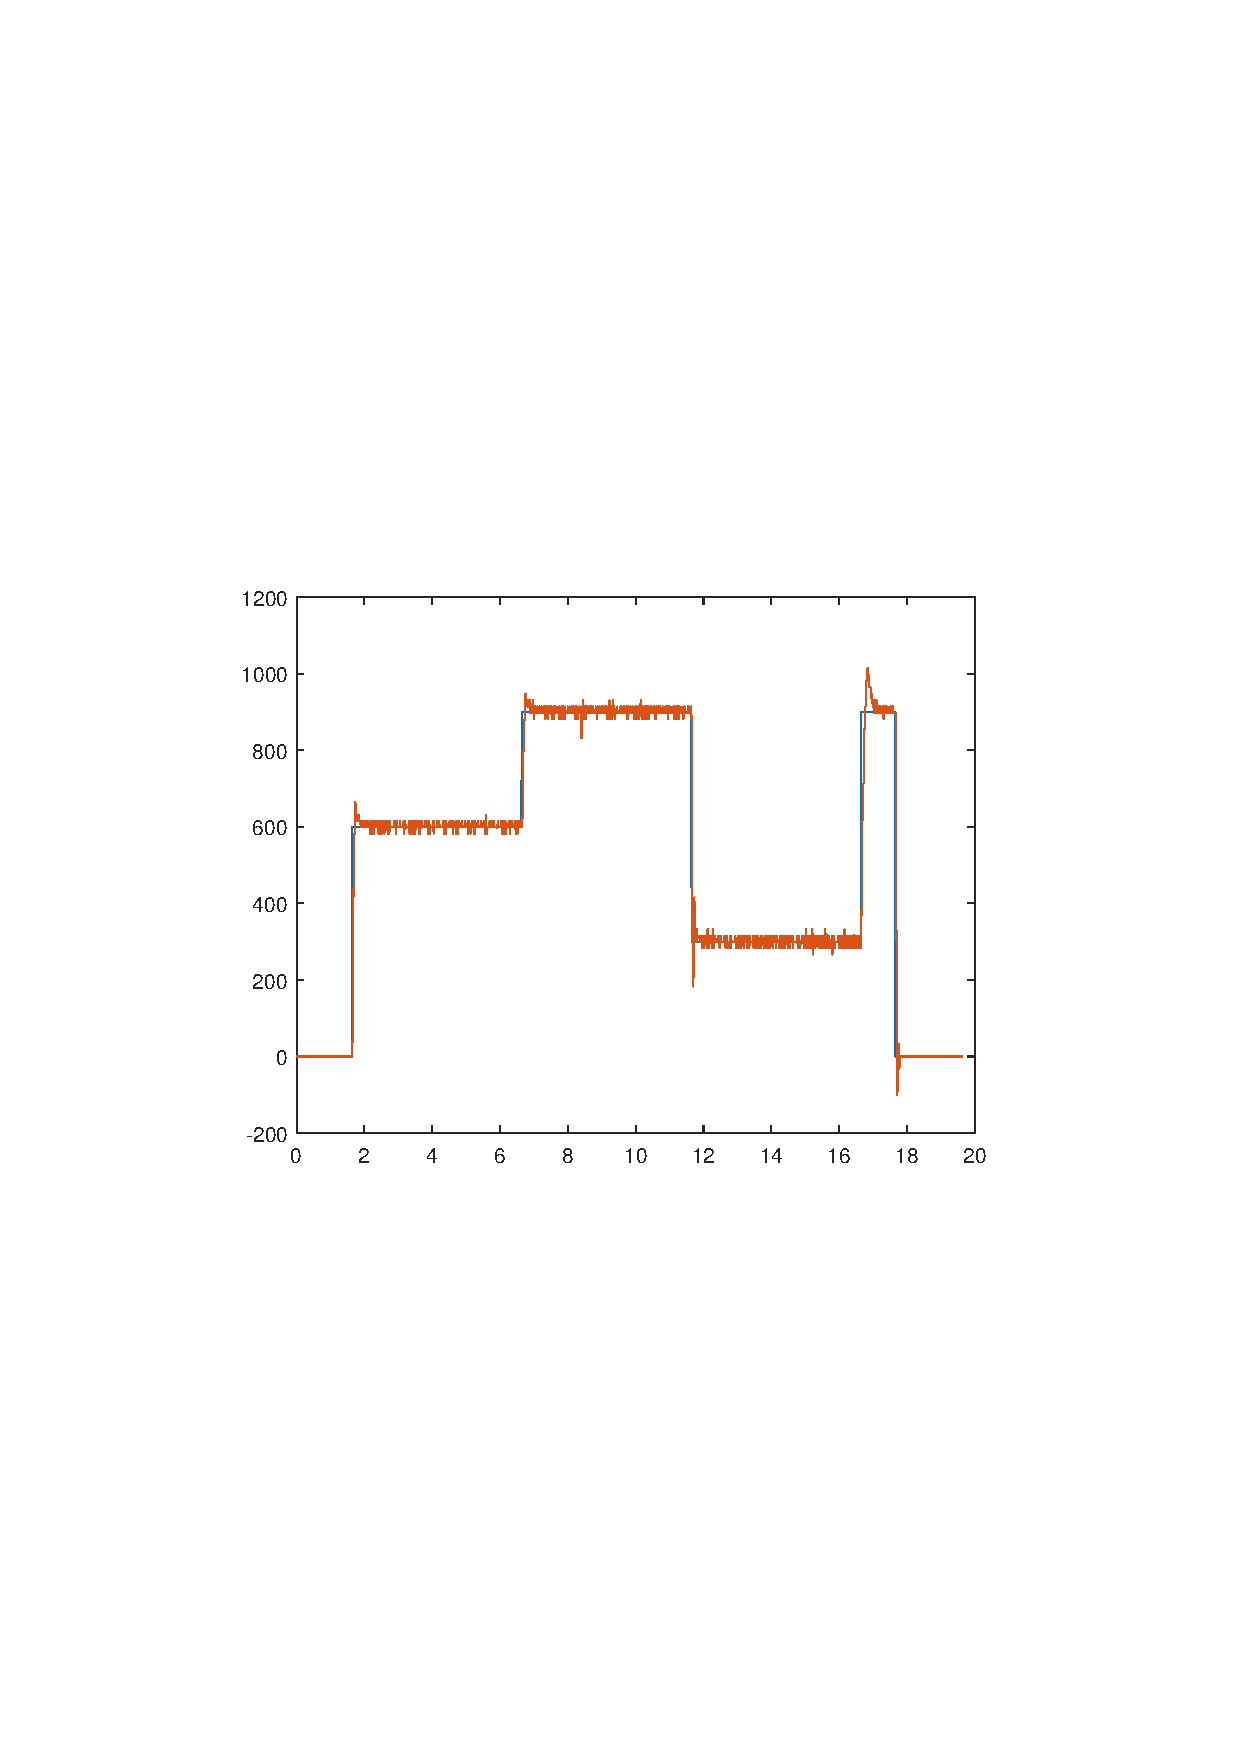
\includegraphics[width=0.8\linewidth]{local-5ms.pdf}
	\caption{Set-point and feedback value curves for local control with 5ms network cycle time}
	\label{fig:local-5ms}
\end{figure}

\subsection{Remote control mode, 5ms network cycle time}

\begin{figure}[htp]
	\centering
	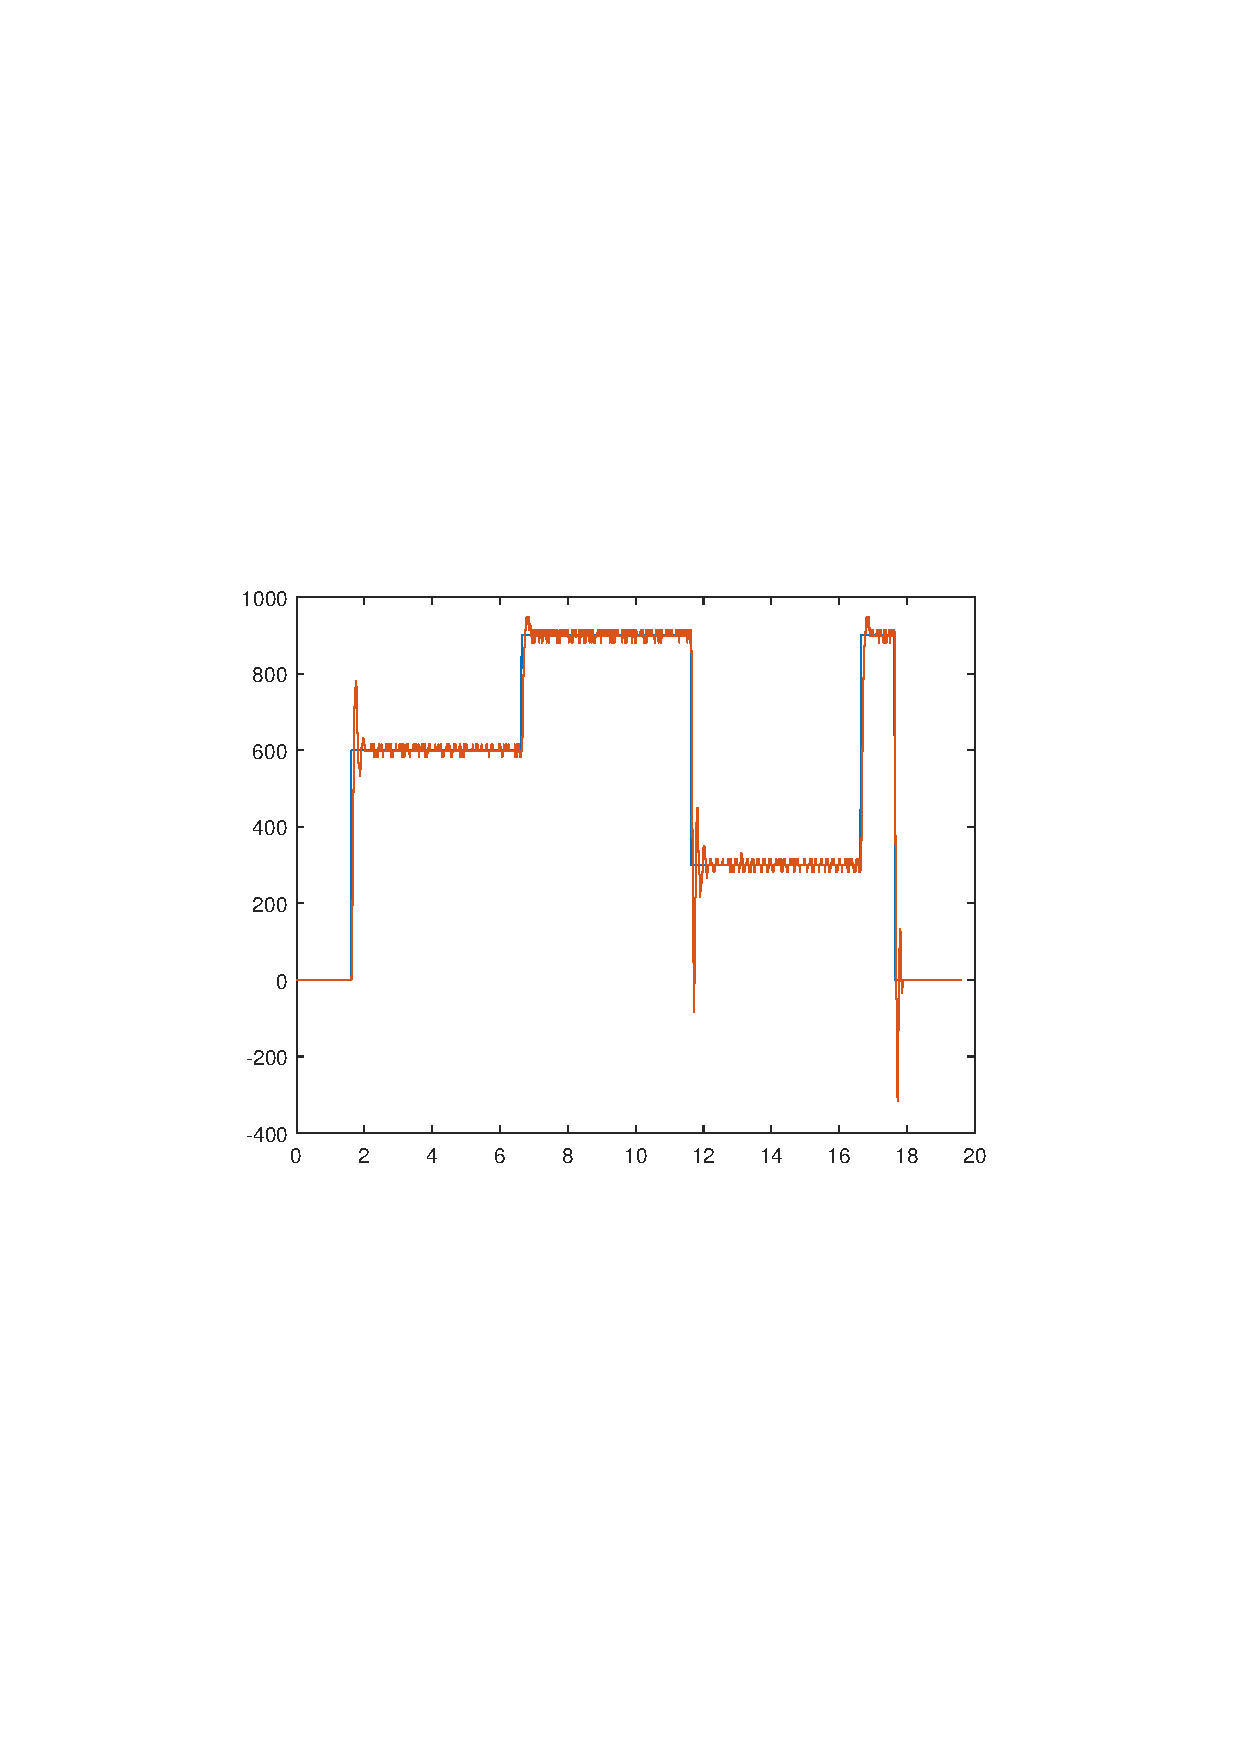
\includegraphics[width=0.8\linewidth]{remote-5ms.pdf}
	\caption{Set-point and feedback value curves for remote control with 5ms network cycle time}
	\label{fig:remote-5ms}
\end{figure}

\subsection{Local control mode, 10ms network cycle time}

\begin{figure}[htp]
	\centering
	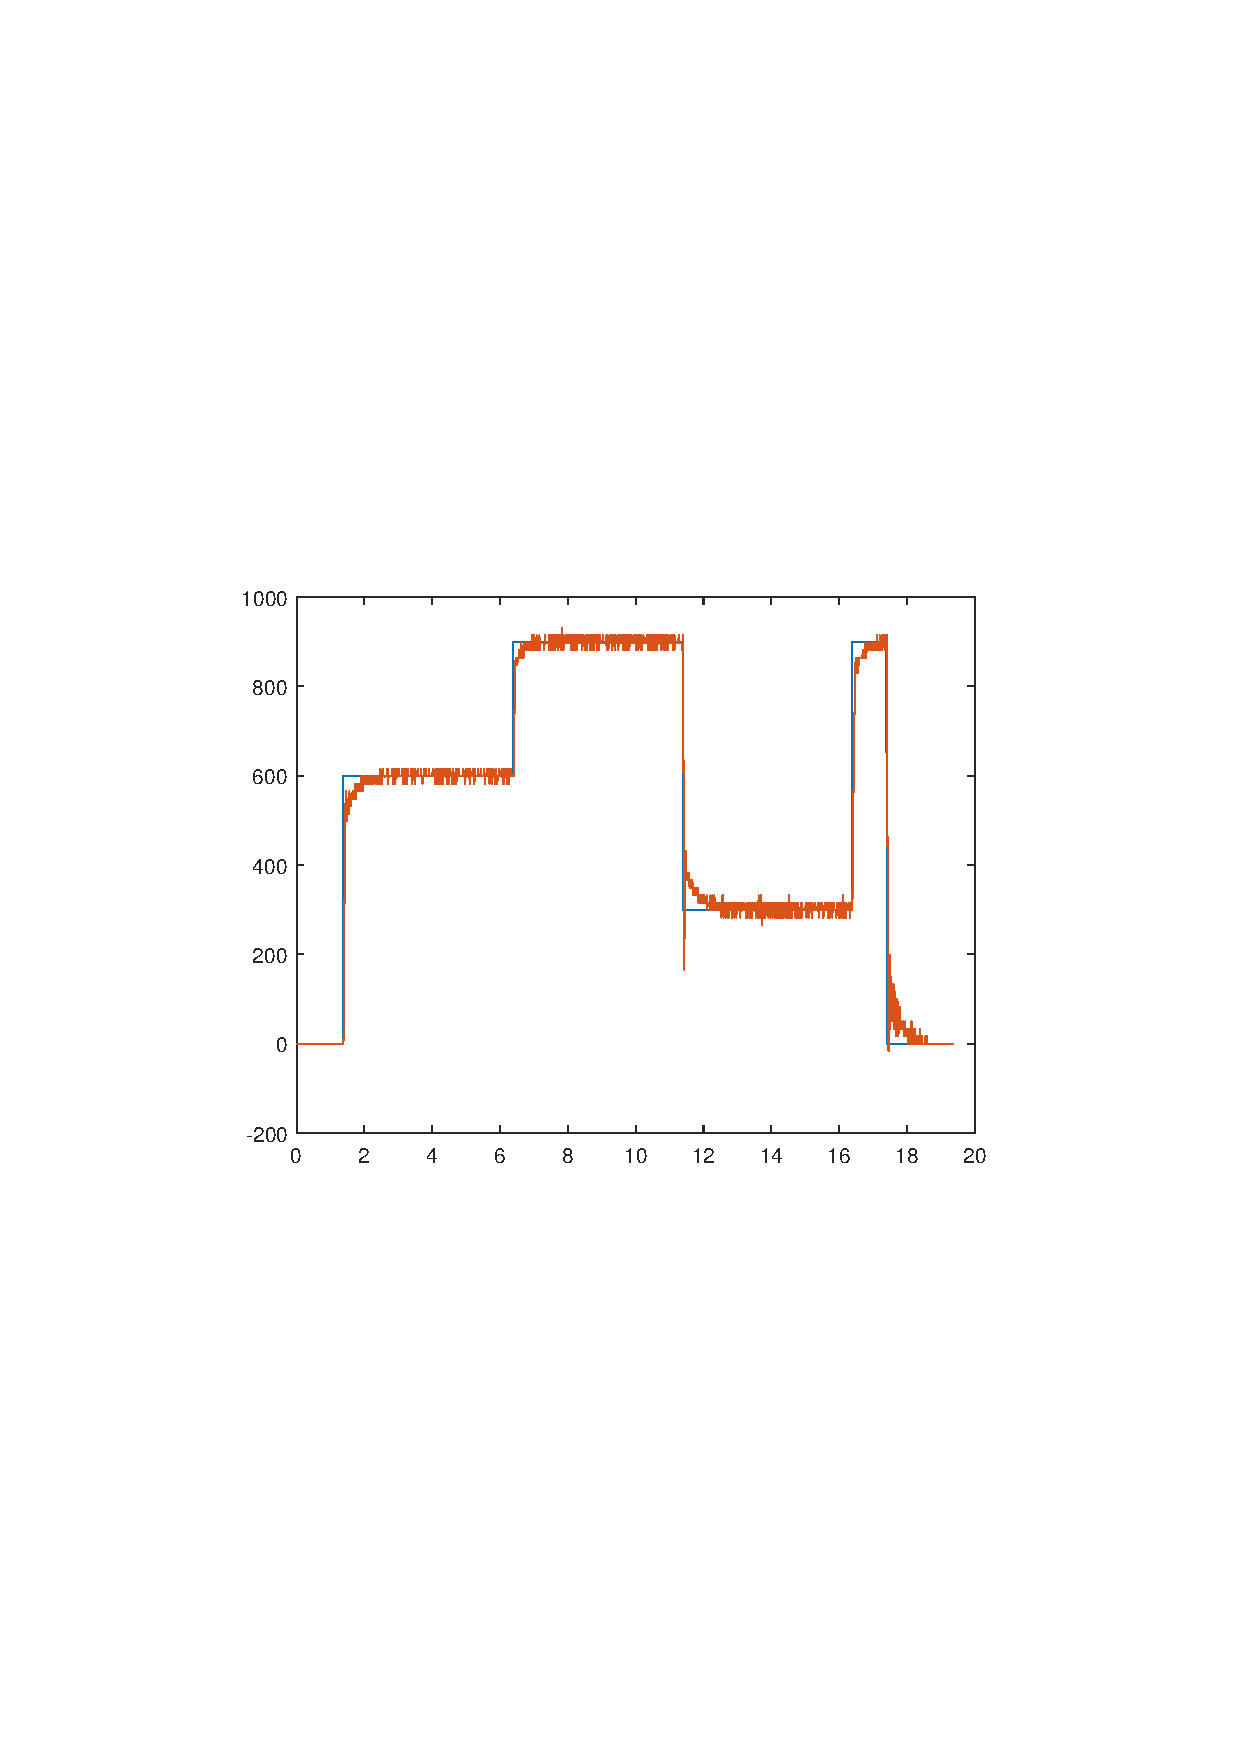
\includegraphics[width=0.8\linewidth]{local-10ms.pdf}
	\caption{Set-point and feedback value curves for local control with 10ms network cycle time}
	\label{fig:local-10ms}
\end{figure}

\subsection{Remote control mode, 10ms network cycle time}

\begin{figure}[htp]
	\centering
	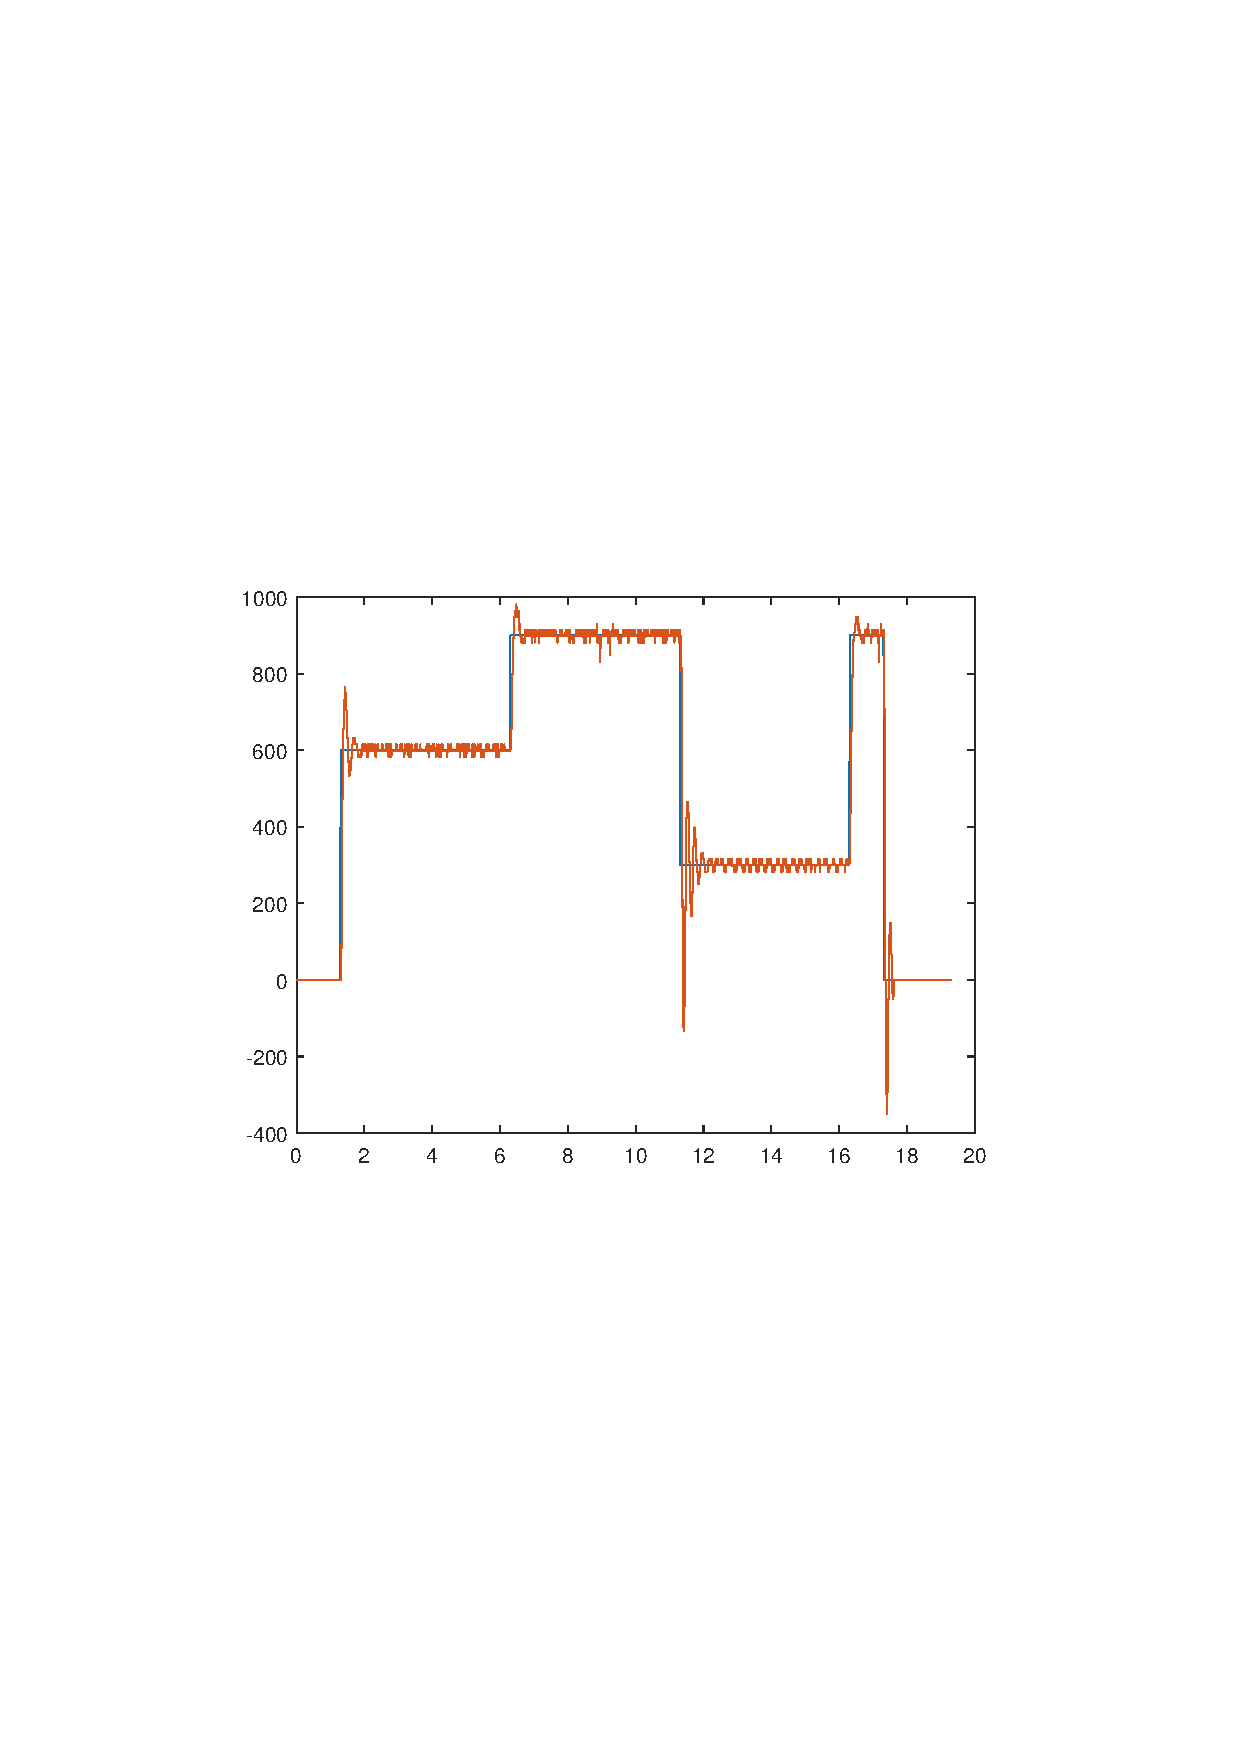
\includegraphics[width=0.8\linewidth]{remote-10ms.pdf}
	\caption{Set-point and feedback value curves for remote control with 10ms network cycle time}
	\label{fig:remote-10ms}
\end{figure}

\subsection{Local control mode, 20ms network cycle time}

\begin{figure}[htp]
	\centering
	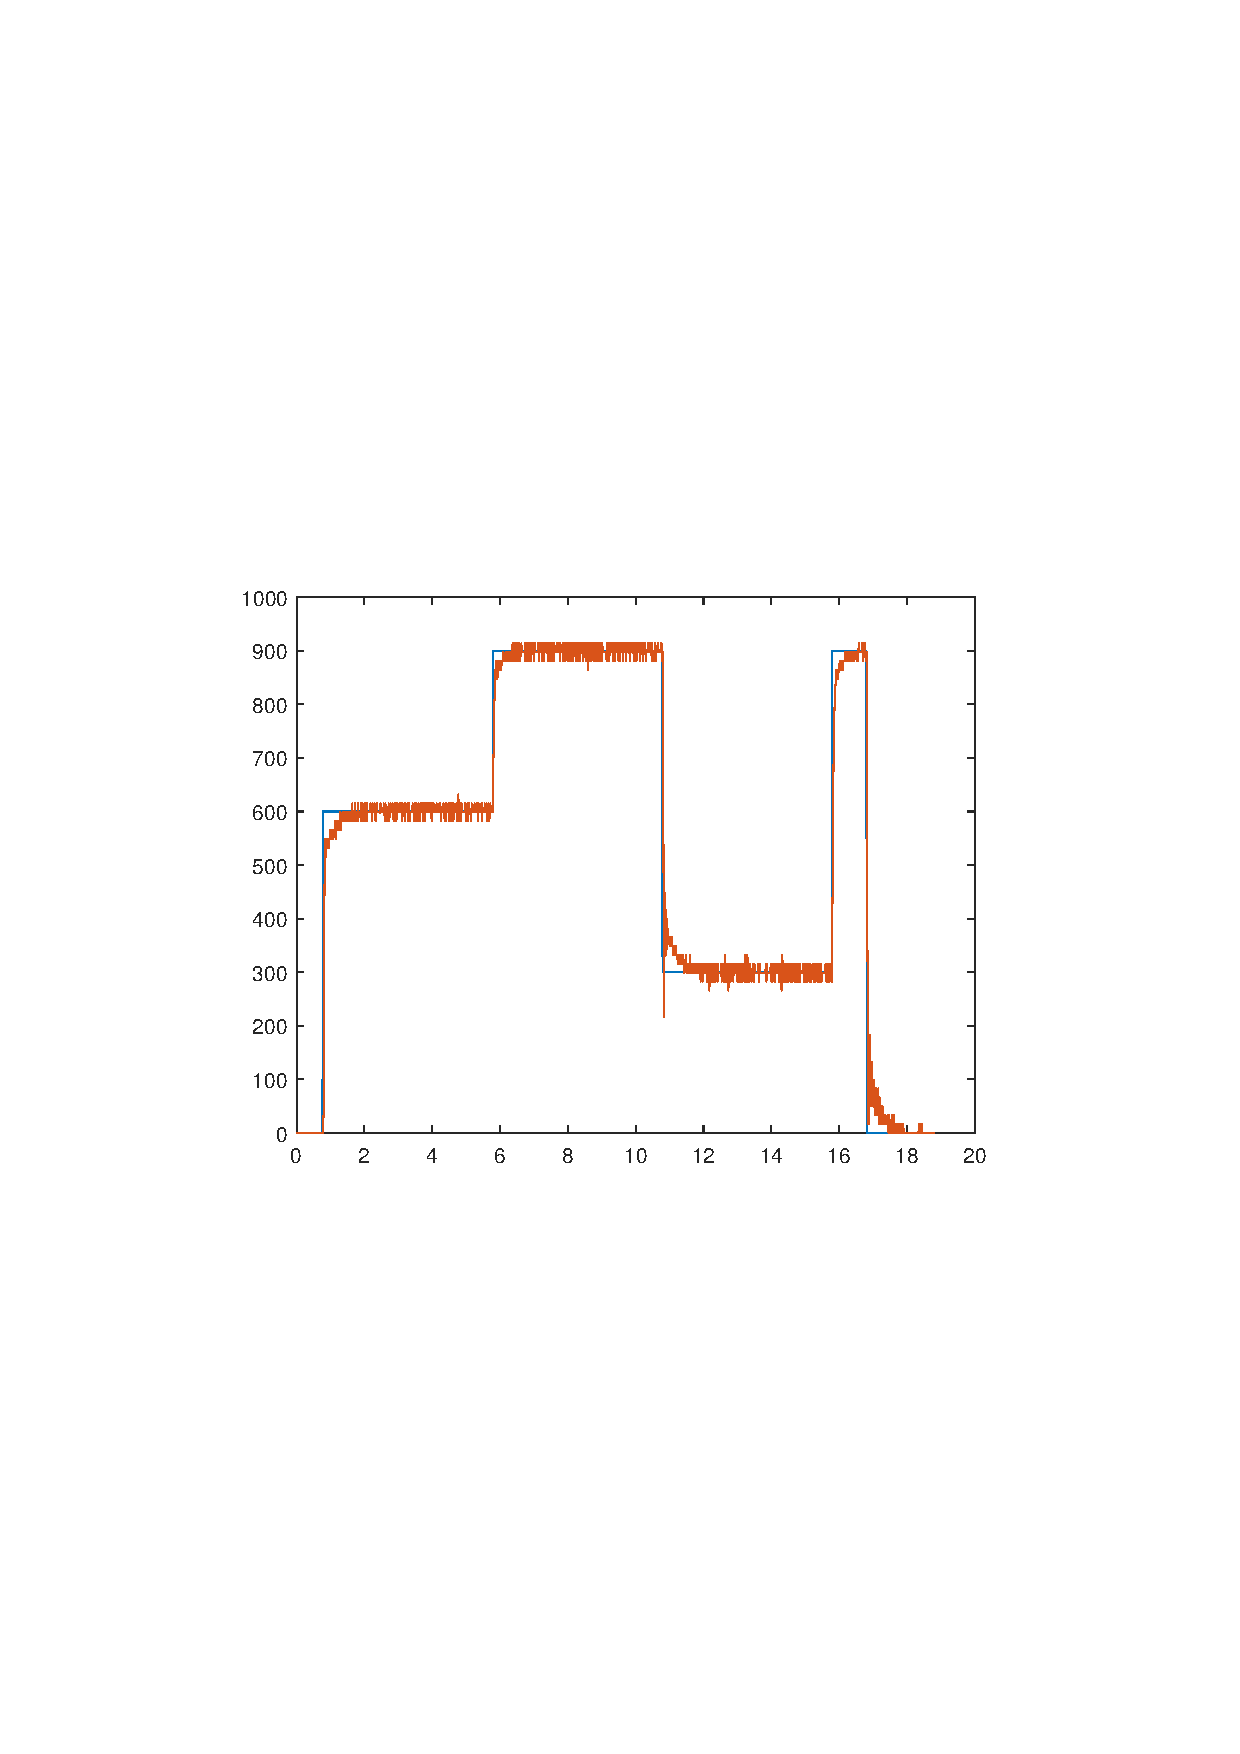
\includegraphics[width=0.8\linewidth]{local-20ms.pdf}
	\caption{Set-point and feedback value curves for local control with 20ms network cycle time}
	\label{fig:local-20ms}
\end{figure}

\subsection{Remote control mode, 20ms network cycle time}

\begin{figure}[htp]
	\centering
	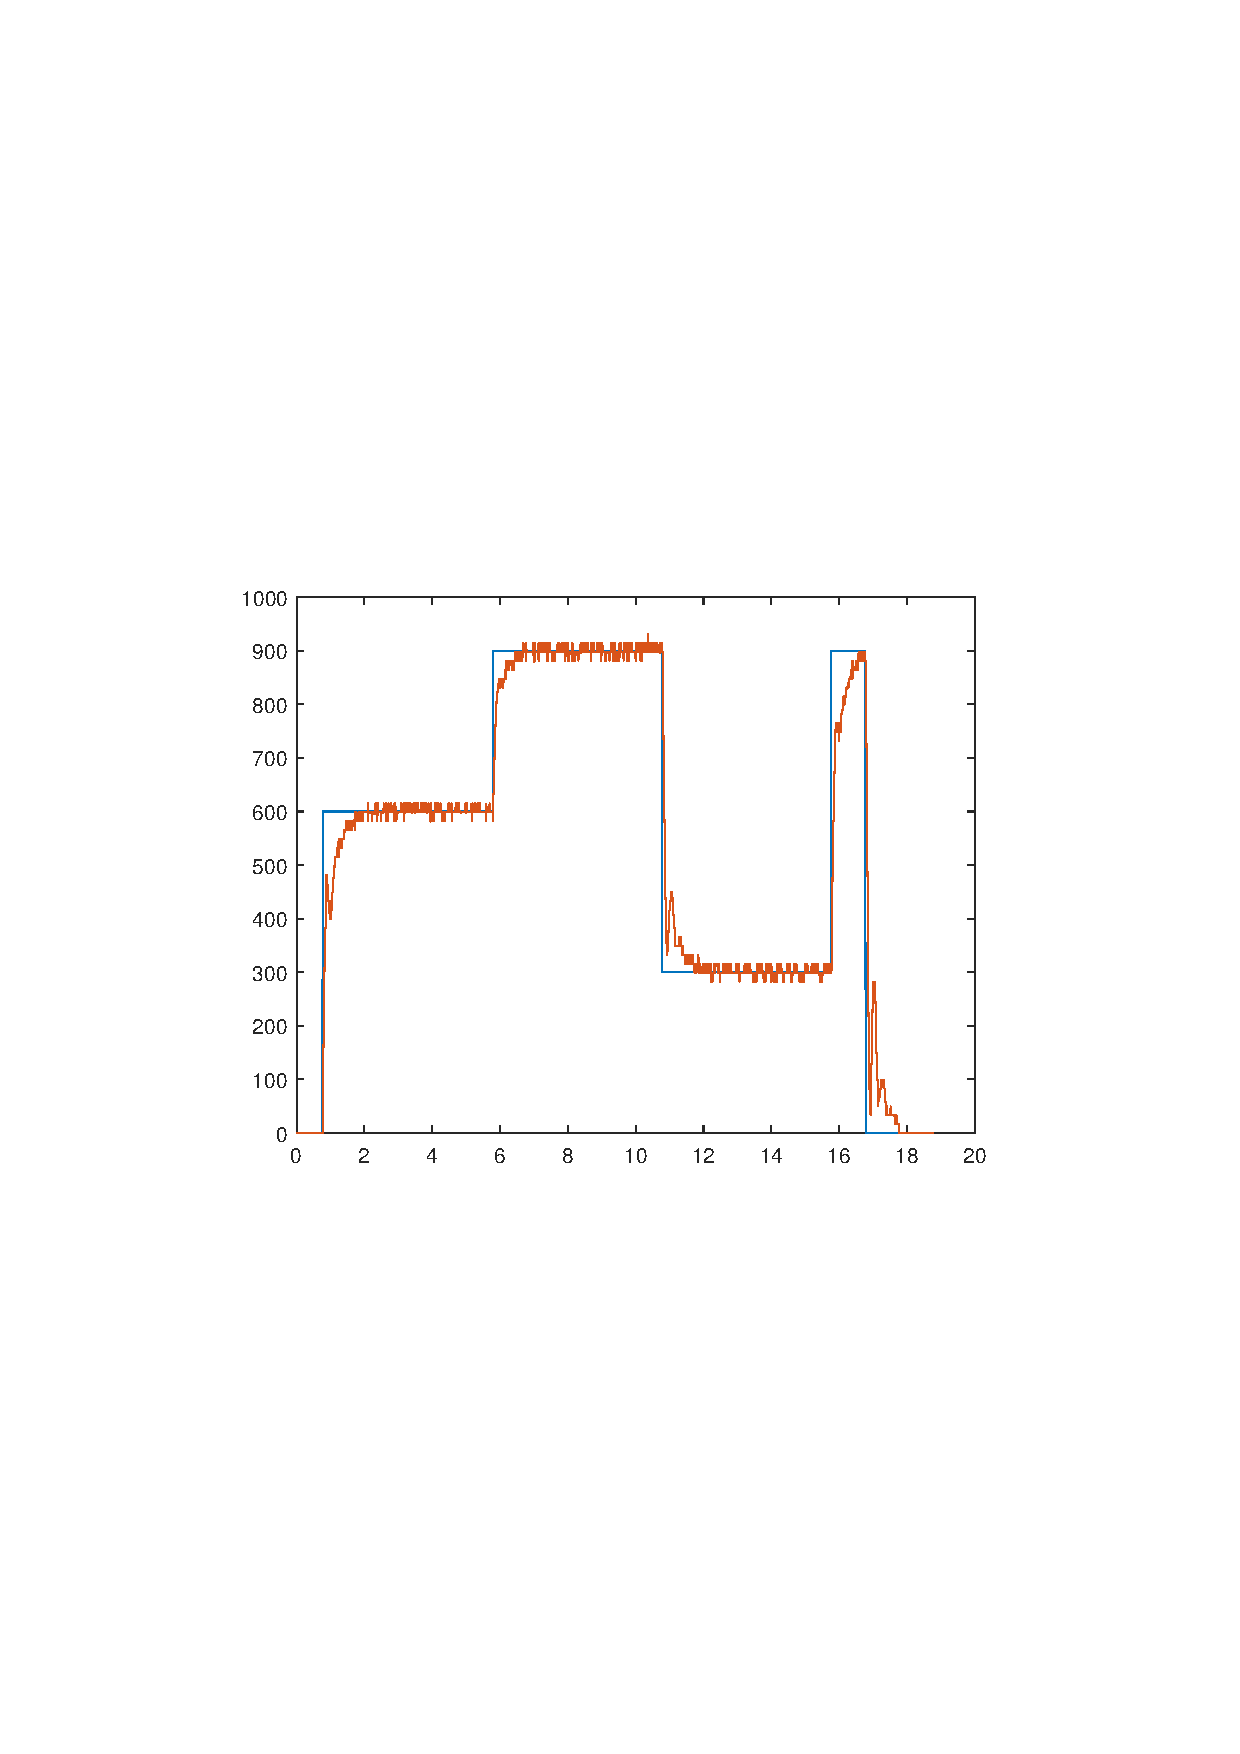
\includegraphics[width=0.8\linewidth]{remote-20ms.pdf}
	\caption{Set-point and feedback value curves for remote control with 20ms network cycle time}
	\label{fig:remote-20ms}
\end{figure}

\subsection{Data analysis}

\begin{table}[htp]
	\centering
	\caption{Encoder step sequence mapping}
	\begin{tabular}{|c|c|c|c|c|c|}
		\hline
		Test Case   & rise-time & settling-time & overshoot & peak & peak time  \\
		\hline
		local-5ms   &           &               &           &      &            \\
		\hline
		remote-5ms  &           &               &           &      &            \\
		\hline
		local-10ms  &           &               &           &      &            \\
		\hline
		remote-10ms &           &               &           &      &            \\
		\hline
		local-20ms  &           &               &           &      &            \\
		\hline
		remote-20ms &           &               &           &      &            \\
		\hline
	\end{tabular}
\end{table}
